In this section, we test our approximation on the Bike-Sharing
Dataset~\cite{BikeSharing}.~\footnote{It is dataset drawn from the
  Capital Bikeshare system (Washington D.C., USA) over the period
  2011-2012. The dataset can be found
  \href{https://archive.ics.uci.edu/ml/machine-learning-databases/00275/Bike-Sharing-Dataset.zip}{here}}
The Bike-Sharing Dataset is chosen as the main illustration example in
the original ALE paper, therefore it was considered appropriate for
comparisons. The dataset contains the bike rentals for almost every
hour over the period 2011 and 2012. The dataset contains 14 features,
which we denote as \( X_{\mathtt{<feature\_name>}} \). We select the
11 features that are relevant to the prediction task. Most of the
features are measurements of the environmental conditions, e.g.
\(X_{\mathtt{month}}\), \(X_{\mathtt{hour}}\),
\(X_{\mathtt{temperature}}\), \(X_{\mathtt{humidity}}\),
\(X_{\mathtt{windspeed}}\), while some others inform us about the
day-type, e.g. whether we refer to a working-day
\(X_{\mathtt{workingday}}\). The target value \( Y_{\mathtt{count}}\)
is the bike rentals per hour, which has mean value
\(\mu_{\mathtt{count}} = 189\) and standard deviation
\(\sigma_{\mathtt{count}} = 181\). We train a deep fully-connected
Neural Network with 6 hidden layers and \(711681\) parameters. We
train the model for \(20\) epochs, using the Adam optimizer with
learning rate 0.01. The model achieves a mean absolute error on the
test of about \(38\) counts.

\paragraph{Efficiency} For comparing the efficiency, we measure the
execution time of DALE and ALE for a variable number of features. We
present the results in Table~\ref{tab:bike-sharing-efficiency}. We
confirm that DALE can compute the feature effect for all features in
almost constant time wrt \(D\). In contrast, ALE scales linearly wrt
\(D\) which leads to an execution time of over \(10\) seconds.

\begin{table}
  \caption{Measurements of the execution time in seconds, for DALE and ALE approximation
    on the Bike Sharing dataset.}
  \label{tab:bike-sharing-efficiency}
  \centering
  \begin{tabular}{c|c|c|c|c|c|c|c|c|c|c|c}
    \multicolumn{12}{c}{Efficiency on Bike-Sharing Dataset} \\
    \hline\hline
    & \multicolumn{11}{|c}{Number of Features} \\
    \hline
    & 1 & 2 & 3 & 4 & 5 & 6 & 7 & 8 & 9 & 10 & 11 \\
    \hline
    \( \dale \) & 1.17 & \textbf{1.19} & \textbf{1.22} & \textbf{1.24} & \textbf{1.27} & \textbf{1.30} & \textbf{1.36} & \textbf{1.32} & \textbf{1.33} & \textbf{1.37} & \textbf{1.39} \\
    \hline
    \( \alep \) & \textbf{0.85} & 1.78 & 2.69 & 3.66 & 4.64 & 5.64 & 6.85 & 7.73 & 8.86 & 9.9 & 10.9 \\
    \hline
  \end{tabular}
\end{table}

\paragraph{Accuracy}

In the case of the Bike-Sharing, it is infeasible compare to compute
the ground-truth ALE. We have lack of knowledge about the
data-generating distribution and the dimensionality of the problem
\(D=11\) is prohibitive for applying numerical integration on
eq.~\eqref{eq:ALE}. However, given the fact that the dataset has a
large number of instances, DALE and ALE provide very similar
approximations for large \(K\), e.g. (\(K=200\)), and we can treat
these approximations as the ground-truth effect. In
Figure~\ref{fig:bike-sharing-comparison}, we illustrate the feature
effect for three features.

For all feature features, except \(X_{\mathtt{hour}}\), lowering the
number of bins \(K\) does not significantly impacts the approximation,
since these features change slowly wrt the feature value. An exception
is feature \(X_{\mathtt{hour}}\). In this case, the
\(f_{\mathtt{DALE}}\) approximation remains accurate when lowering the
number of bins \(K\) (Fig.~\ref{fig:bike-sharing-feature-3}(b)), while
\(\hat{f}_{\mathtt{ALE}}\) deteriorates significantly
(Fig.~\ref{fig:bike-sharing-feature-3}(c)). In
Table~\ref{tab:bike-sharing-accuracy} we evaluate the feature effect
of \(X_{\mathtt{hour}}\) for different number of bins \(K\). The
ground-truth effect has been computed for \(K=200\). We observe that
NMSE remains low in DALE for all \(K\), while for ALE it rapidly
increases. This is due to OOD sampling that occurs when the bin size
becomes large.


\begin{figure}[h]
  \centering
  \resizebox{.3\columnwidth}{!}{% This file was created with tikzplotlib v0.10.1.
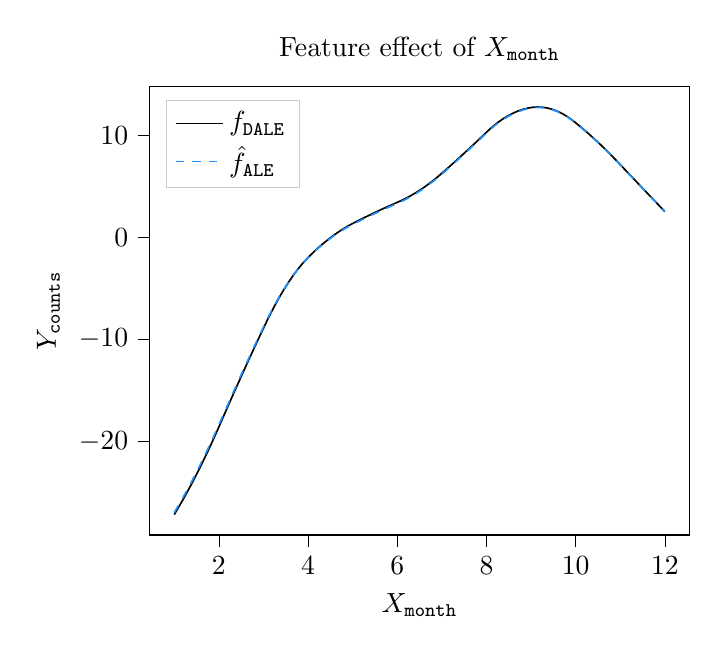
\begin{tikzpicture}

\definecolor{darkgray176}{RGB}{176,176,176}
\definecolor{dodgerblue}{RGB}{30,144,255}
\definecolor{lightgray204}{RGB}{204,204,204}

\begin{axis}[
legend cell align={left},
legend style={
  fill opacity=0.8,
  draw opacity=1,
  text opacity=1,
  at={(0.03,0.97)},
  anchor=north west,
  draw=lightgray204
},
tick align=outside,
tick pos=left,
title={Feature effect of \(\displaystyle X_{\mathtt{month}}\)},
x grid style={darkgray176},
xlabel={\(\displaystyle X_{\mathtt{month}}\)},
xmin=0.45, xmax=12.55,
xtick style={color=black},
y grid style={darkgray176},
ylabel={\(\displaystyle Y_{\mathtt{counts}}\)},
ymin=-29.183798458369, ymax=14.7468616660552,
ytick style={color=black}
]
\addplot [semithick, black]
table {%
1 -27.1869506835938
1.17617619037628 -25.871150970459
1.29729723930359 -24.9201946258545
1.40740740299225 -24.0201549530029
1.51751756668091 -23.0867099761963
1.63863861560822 -22.0221939086914
1.74874877929688 -21.0186061859131
1.85885882377625 -19.9816131591797
1.9689689874649 -18.9112167358398
2.09009003639221 -17.6963996887207
2.32132124900818 -15.3969707489014
2.64064073562622 -12.2988424301147
2.87187194824219 -10.1101322174072
3.1141140460968 -7.87898731231689
3.24624633789062 -6.75733757019043
3.35635638237 -5.88665103912354
3.45545554161072 -5.15343141555786
3.56556558609009 -4.3964409828186
3.67567563056946 -3.69928789138794
3.77477478981018 -3.12166857719421
3.88488483428955 -2.53821158409119
3.99499487876892 -2.01459169387817
4.13813829421997 -1.40747404098511
4.23723745346069 -1.0118283033371
4.34734725952148 -0.59662914276123
4.45745754241943 -0.207057595252991
4.56756734848022 0.156886339187622
4.66666650772095 0.462822675704956
4.7767767906189 0.778071641921997
4.88688707351685 1.06769299507141
4.98598575592041 1.30698728561401
5.21721744537354 1.81831657886505
5.43743753433228 2.28735709190369
5.64664649963379 2.71674489974976
5.86686706542969 3.15148568153381
6.12012004852295 3.64487433433533
6.19719696044922 3.81250214576721
6.30730724334717 4.07315158843994
6.42842864990234 4.38769626617432
6.53853845596313 4.69808197021484
6.64864873886108 5.03215312957764
6.75875854492188 5.3899097442627
6.87987995147705 5.81102657318115
6.98998975753784 6.21852016448975
7.23223209381104 7.15501070022583
7.463463306427 8.071533203125
7.6836838722229 8.96508026123047
7.90390396118164 9.87869548797607
8.09109115600586 10.6491012573242
8.17917919158936 10.9760904312134
8.27827835083008 11.3111982345581
8.38838863372803 11.6416292190552
8.49849891662598 11.9293622970581
8.60860824584961 12.1743965148926
8.70770740509033 12.3600397109985
8.81781768798828 12.5239429473877
8.92792797088623 12.6451482772827
9.03803825378418 12.7230014801025
9.1371374130249 12.7500133514404
9.17016983032227 12.7448768615723
9.24724769592285 12.7297611236572
9.28028011322021 12.7090911865234
9.35735702514648 12.6578493118286
9.40140151977539 12.6091642379761
9.47847843170166 12.5178241729736
9.58858871459961 12.3373823165894
9.69869899749756 12.1052808761597
9.80880928039551 11.8215208053589
9.92992973327637 11.4478168487549
10.1061058044434 10.8241405487061
10.2162160873413 10.4159374237061
10.3263263702393 9.99349880218506
10.4364366531372 9.55682373046875
10.5575571060181 9.06051921844482
10.667667388916 8.59395122528076
10.777777671814 8.11314868927002
10.8988990783691 7.56844854354858
11.7247247695923 3.76278614997864
12 2.50704598426819
};
\addlegendentry{$f_{\mathtt{DALE}}$}
\addplot [semithick, dodgerblue, dashed]
table {%
1 -27.0010604858398
1.18718719482422 -25.586950302124
1.29729723930359 -24.7142314910889
1.40740740299225 -23.809778213501
1.52852857112885 -22.77903175354
1.63863861560822 -21.8079357147217
1.74874877929688 -20.8051052093506
1.86986982822418 -19.666467666626
1.99099099636078 -18.4894695281982
2.2992992401123 -15.4285402297974
2.51951956748962 -13.2975368499756
2.72872877120972 -11.3166017532349
2.94894886016846 -9.27656745910645
3.1141140460968 -7.78738117218018
3.24624633789062 -6.68413352966309
3.35635638237 -5.82812023162842
3.45545554161072 -5.10758543014526
3.56556558609009 -4.36409330368042
3.67567563056946 -3.67981958389282
3.77477478981018 -3.113276720047
3.88488483428955 -2.54152417182922
3.99499487876892 -2.02899026870728
4.13813829421997 -1.43530428409576
4.23723745346069 -1.04830312728882
4.34734725952148 -0.642061471939087
4.45745754241943 -0.260767459869385
4.56756734848022 0.0955789089202881
4.66666650772095 0.395250797271729
4.7767767906189 0.704194068908691
4.88688707351685 0.988189816474915
4.98598575592041 1.22298789024353
5.23923921585083 1.77311503887177
5.4484486579895 2.21300554275513
5.66866874694824 2.66170525550842
5.88888883590698 3.09569883346558
6.10910892486572 3.52712678909302
6.19719696044922 3.71933627128601
6.30730724334717 3.9817156791687
6.42842864990234 4.29802989959717
6.53853845596313 4.60990715026855
6.64864873886108 4.9453558921814
6.75875854492188 5.30437612533569
6.87987995147705 5.72675085067749
6.98998975753784 6.13526916503906
7.24324321746826 7.11681127548218
7.463463306427 7.99168014526367
7.6836838722229 8.8862886428833
7.90390396118164 9.80063629150391
8.09109115600586 10.5716905593872
8.17917919158936 10.899432182312
8.2892894744873 11.2697401046753
8.38838863372803 11.5681610107422
8.49849891662598 11.8583631515503
8.60860824584961 12.106406211853
8.70770740509033 12.2951984405518
8.81781768798828 12.463134765625
8.92792797088623 12.5889139175415
9.03803825378418 12.6718053817749
9.1371374130249 12.702956199646
9.17016983032227 12.6990699768066
9.24724769592285 12.6868410110474
9.28028011322021 12.6672773361206
9.35735702514648 12.6185913085938
9.40140151977539 12.5711889266968
9.47847843170166 12.4820346832275
9.58858871459961 12.3042573928833
9.69869899749756 12.0743465423584
9.80880928039551 11.7923011779785
9.92992973327637 11.4199190139771
10.1061058044434 10.7974834442139
10.2162160873413 10.3899793624878
10.3263263702393 9.96817970275879
10.4364366531372 9.53208541870117
10.5575571060181 9.03635120391846
10.667667388916 8.57023906707764
10.777777671814 8.08983135223389
10.8988990783691 7.54549980163574
11.7027025222778 3.84338307380676
12 2.48848509788513
};
\addlegendentry{$\hat{f}_{\mathtt{ALE}}$}
\end{axis}

\end{tikzpicture}
}
  \resizebox{.3\columnwidth}{!}{% This file was created with tikzplotlib v0.10.1.
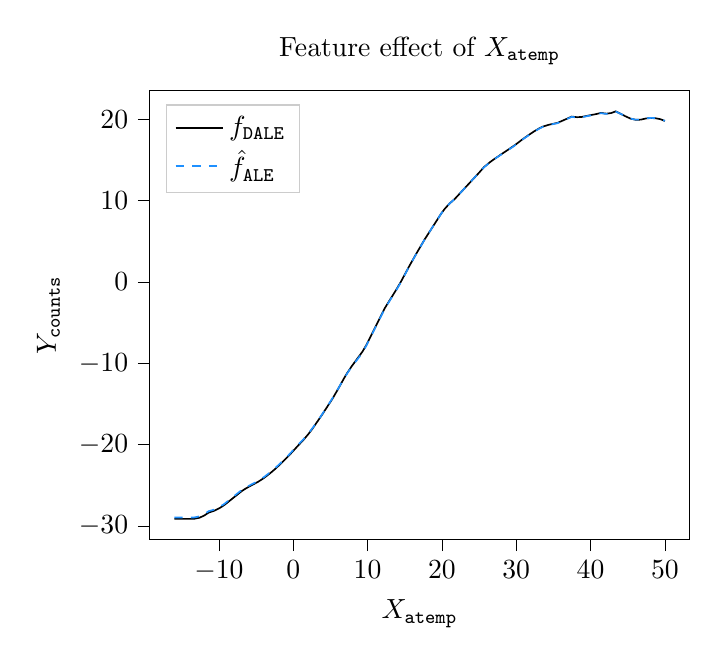
\begin{tikzpicture}

\definecolor{darkgray176}{RGB}{176,176,176}
\definecolor{dodgerblue}{RGB}{30,144,255}
\definecolor{lightgray204}{RGB}{204,204,204}

\begin{axis}[
legend cell align={left},
legend style={
  fill opacity=0.8,
  draw opacity=1,
  text opacity=1,
  at={(0.03,0.97)},
  anchor=north west,
  draw=lightgray204
},
tick align=outside,
tick pos=left,
title={Feature effect of \(\displaystyle X_{\mathtt{atemp}}\)},
x grid style={darkgray176},
xlabel={\(\displaystyle X_{\mathtt{atemp}}\)},
xmin=-19.3, xmax=53.3,
xtick style={color=black},
y grid style={darkgray176},
ylabel={\(\displaystyle Y_{\mathtt{counts}}\)},
ymin=-31.6301535780892, ymax=23.4795271752803,
ytick style={color=black}
]
\addplot [semithick, black]
table {%
-16 -29.1201610565186
-14.5465469360352 -29.1236610412598
-13.3573570251465 -29.1187324523926
-12.6306304931641 -28.9887657165527
-11.9699697494507 -28.7167987823486
-11.3753757476807 -28.351110458374
-10.5825824737549 -28.10817527771
-9.9219217300415 -27.8089466094971
-9.26126098632812 -27.4157428741455
-8.13813781738281 -26.5979690551758
-6.94894886016846 -25.7284774780273
-6.55255270004272 -25.4859237670898
-5.89189195632935 -25.1317119598389
-4.70270252227783 -24.557861328125
-3.90990996360779 -24.0795192718506
-3.11711716651917 -23.5240688323975
-2.52252244949341 -23.0663394927979
-1.86186182498932 -22.5092353820801
-0.540540456771851 -21.3122959136963
0.120120167732239 -20.6509094238281
0.714714765548706 -20.0558643341064
1.30930936336517 -19.4900760650635
2.03603601455688 -18.7049884796143
2.63063073158264 -17.9895362854004
3.8858859539032 -16.3134365081787
5.27327346801758 -14.3682708740234
6 -13.2194204330444
6.85885906219482 -11.8082704544067
7.25525522232056 -11.203857421875
7.91591596603394 -10.3020009994507
9.30330371856689 -8.58228397369385
9.83183193206787 -7.77181529998779
10.9549551010132 -5.72904586791992
12.342342376709 -3.19349336624146
12.5405406951904 -2.89349699020386
13.7957954406738 -1.05008816719055
14.4564561843872 -0.0256915092468262
15.6456460952759 2.00035262107849
16.5705699920654 3.49347949028015
17.6936931610107 5.24578619003296
19.9399394989014 8.44653511047363
20.4024028778076 9.01027202606201
21.0630626678467 9.66129207611084
21.7237243652344 10.1941547393799
24.8948955535889 13.3221054077148
25.687686920166 14.134651184082
26.4804801940918 14.7308025360107
27.1411418914795 15.1683645248413
29.8498497009277 16.8362903594971
30.7087078094482 17.4392356872559
31.3693695068359 17.8697376251221
32.3603591918945 18.484224319458
33.087085723877 18.8724536895752
33.5495491027832 19.0880432128906
34.4084091186523 19.3274822235107
35.0690689086914 19.4596900939941
35.5315322875977 19.543493270874
36.9849853515625 20.1296157836914
37.4474487304688 20.3274917602539
37.6456451416016 20.3095550537109
38.1741752624512 20.2521419525146
38.8348350524902 20.287296295166
39.8258247375488 20.4710922241211
40.6186180114746 20.6114158630371
41.345344543457 20.7675323486328
41.4114112854004 20.7821464538574
41.8078079223633 20.7240734100342
42.1381378173828 20.6876392364502
42.7987976074219 20.7667903900146
43.3933944702148 20.9745426177979
43.657657623291 20.8512020111084
44.714714050293 20.3551597595215
45.4414405822754 20.057201385498
46.1021003723145 19.9324207305908
46.7627639770508 19.9523639678955
47.4894905090332 20.1014881134033
48.1501502990723 20.1500225067139
48.8108100891113 20.1130447387695
49.4054069519043 20.0048065185547
50 19.7889881134033
};
\addlegendentry{$f_{\mathtt{DALE}}$}
\addplot [semithick, dodgerblue, dashed]
table {%
-16 -28.9542388916016
-14.5465469360352 -28.9578762054443
-13.3573570251465 -28.9526977539062
-12.6306304931641 -28.8202018737793
-11.9699697494507 -28.5466842651367
-11.3753757476807 -28.1803741455078
-10.6486482620239 -27.9906787872314
-9.98798751831055 -27.7104911804199
-9.26126098632812 -27.2779521942139
-8.00600624084473 -26.3645648956299
-7.2132134437561 -25.7814712524414
-6.55255270004272 -25.3670864105225
-5.89189195632935 -25.0190086364746
-4.76876878738403 -24.4896812438965
-3.90990996360779 -23.9704494476318
-3.05105113983154 -23.364631652832
-2.52252244949341 -22.9567375183105
-1.86186182498932 -22.4021339416504
-0.606606602668762 -21.2720623016357
0.120120167732239 -20.5483741760254
0.648648619651794 -20.0188083648682
1.30930936336517 -19.4072608947754
1.96996998786926 -18.7101631164551
2.69669675827026 -17.8467922210693
3.55555558204651 -16.7303333282471
4.21621608734131 -15.8174858093262
5.53753757476807 -13.9267387390137
6 -13.1932601928711
6.66066074371338 -12.1299390792847
7.32132148742676 -11.1632461547852
7.91591596603394 -10.3738870620728
8.97297286987305 -9.1130838394165
9.10510540008545 -8.9506664276123
9.83183193206787 -7.83912706375122
11.2852849960327 -5.17018270492554
12.408408164978 -3.13905572891235
13.5975971221924 -1.41476833820343
14.3243246078491 -0.306623458862305
14.6546545028687 0.264089107513428
15.6456460952759 1.96240651607513
16.5705699920654 3.46715188026428
17.6936931610107 5.24065256118774
19.8738746643066 8.35614967346191
20.4024028778076 9.0117301940918
21.0630626678467 9.66457653045654
21.7237243652344 10.1938533782959
25.4894886016846 13.9263477325439
25.6216220855713 14.053521156311
26.4804801940918 14.7064094543457
27.1411418914795 15.1473188400269
29.057056427002 16.3006134033203
29.6516513824463 16.6701507568359
30.6426429748535 17.3715686798096
31.2372379302979 17.7557601928711
32.4924926757812 18.524055480957
33.087085723877 18.8392581939697
33.5495491027832 19.0558605194092
34.4084091186523 19.2951412200928
35.0690689086914 19.4283008575439
35.5315322875977 19.5130195617676
36.9849853515625 20.0959377288818
37.4474487304688 20.291877746582
37.6456451416016 20.2738914489746
38.1741752624512 20.216480255127
38.8348350524902 20.2516288757324
39.8258247375488 20.4354114532471
40.6186180114746 20.5759296417236
41.2792778015137 20.7178859710693
41.4114112854004 20.7472190856934
41.8078079223633 20.6907978057861
42.1381378173828 20.6556282043457
42.7987976074219 20.7358493804932
43.3933944702148 20.9432563781738
43.657657623291 20.8323345184326
45.375373840332 20.0885391235352
46.0360374450684 19.9492740631104
46.6966972351074 19.9548187255859
47.5555572509766 20.1251811981201
48.1501502990723 20.1673374176025
48.8108100891113 20.1304454803467
49.4054069519043 20.0222206115723
50 19.8063983917236
};
\addlegendentry{$\hat{f}_{\mathtt{ALE}}$}
\end{axis}

\end{tikzpicture}
}
  \resizebox{.3\columnwidth}{!}{% This file was created with tikzplotlib v0.10.1.
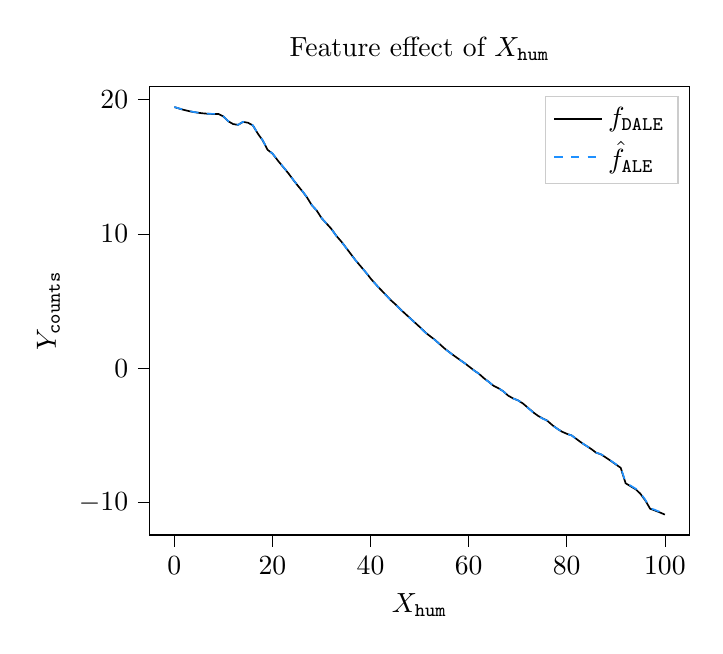
\begin{tikzpicture}

\definecolor{darkgray176}{RGB}{176,176,176}
\definecolor{dodgerblue}{RGB}{30,144,255}
\definecolor{lightgray204}{RGB}{204,204,204}

\begin{axis}[
legend cell align={left},
legend style={fill opacity=0.8, draw opacity=1, text opacity=1, draw=lightgray204},
tick align=outside,
tick pos=left,
title={Feature effect of \(\displaystyle X_{\mathtt{hum}}\)},
x grid style={darkgray176},
xlabel={\(\displaystyle X_{\mathtt{hum}}\)},
xmin=-5, xmax=105,
xtick style={color=black},
y grid style={darkgray176},
ylabel={\(\displaystyle Y_{\mathtt{counts}}\)},
ymin=-12.4017583163331, ymax=20.9680093156312,
ytick style={color=black}
]
\addplot [semithick, black]
table {%
0 19.445671081543
1.80180180072784 19.2508811950684
2.8028028011322 19.1621017456055
3.80380392074585 19.0876598358154
4.80480480194092 19.0275573730469
5.80580568313599 18.9817924499512
6.80680704116821 18.9503650665283
7.80780792236328 18.933277130127
8.80880928039551 18.9305267333984
9.00900936126709 18.9289054870605
10.010009765625 18.7470264434814
11.0110111236572 18.3885173797607
12.0120124816895 18.1801509857178
13.0130128860474 18.1236801147461
14.0140142440796 18.3442001342773
15.0150146484375 18.2827415466309
16.0160160064697 18.0843563079834
17.1171169281006 17.4235782623291
18.0180187225342 16.9714221954346
19.0190181732178 16.268253326416
20.02001953125 15.9827404022217
21.2212219238281 15.4168157577515
23.2232227325439 14.5354175567627
24.4244251251221 13.9460258483887
25.325325012207 13.5335330963135
26.2262268066406 13.1304426193237
27.027027130127 12.738260269165
28.0280284881592 12.1465797424316
29.0290298461914 11.7472257614136
30.030029296875 11.1805286407471
31.9319324493408 10.4186792373657
32.1321334838867 10.3230867385864
33.033031463623 9.86366176605225
34.1341323852539 9.40140438079834
36.9369354248047 8.0537805557251
37.4374389648438 7.83730363845825
39.2392387390137 7.05814123153687
40.1401405334473 6.63687181472778
41.5415420532227 6.06709289550781
42.5425415039062 5.68619441986084
43.3433418273926 5.3793511390686
44.1441459655762 5.07060098648071
45.1451454162598 4.7441782951355
46.2462463378906 4.34106254577637
50.1501502990723 3.03945064544678
51.1511497497559 2.67909049987793
52.352352142334 2.33571791648865
53.1531524658203 2.11605978012085
54.5545539855957 1.6564826965332
55.1551551818848 1.46061563491821
56.6566581726074 1.04154002666473
58.0580596923828 0.674215078353882
59.4594612121582 0.312742352485657
60.4604606628418 0.0281145572662354
61.1611595153809 -0.170746326446533
62.0620613098145 -0.390427708625793
63.1631622314453 -0.749048829078674
64.1641616821289 -1.0204029083252
65.0650634765625 -1.29337751865387
66.1661682128906 -1.49768507480621
67.0670700073242 -1.71112847328186
68.0680694580078 -2.03258061408997
69.0690689086914 -2.23863196372986
70.070068359375 -2.38389420509338
71.0710678100586 -2.61734461784363
73.3733749389648 -3.33057689666748
74.1741714477539 -3.53978538513184
75.175178527832 -3.74607062339783
75.9759750366211 -3.88061666488647
76.3763732910156 -4.00896739959717
77.1771774291992 -4.26187658309937
78.2782745361328 -4.54429483413696
79.0790786743164 -4.72437953948975
80.1801834106445 -4.89549112319946
80.9809799194336 -4.98908805847168
81.3813781738281 -5.09695863723755
82.8828811645508 -5.50094985961914
83.5835800170898 -5.67414093017578
84.584587097168 -5.90682792663574
85.185188293457 -6.05287551879883
85.9859848022461 -6.28149127960205
86.4864883422852 -6.34115266799927
87.0870895385742 -6.42070388793945
88.6886901855469 -6.81395483016968
90.9909896850586 -7.4021258354187
91.2912902832031 -7.73944664001465
91.9919891357422 -8.54510974884033
92.1921920776367 -8.59602737426758
94.0940933227539 -9.01366710662842
94.9949951171875 -9.32887077331543
95.9959945678711 -9.81900787353516
96.9969940185547 -10.4498987197876
97.7977981567383 -10.5560169219971
98.7987976074219 -10.6977682113647
99.7997970581055 -10.85329246521
100 -10.8849506378174
};
\addlegendentry{$f_{\mathtt{DALE}}$}
\addplot [semithick, dodgerblue, dashed]
table {%
0 19.4512023925781
1.80180180072784 19.2567539215088
2.8028028011322 19.1681327819824
3.80380392074585 19.093822479248
4.80480480194092 19.0338249206543
5.80580568313599 18.9881401062012
6.80680704116821 18.9567699432373
7.80780792236328 18.9397106170654
8.80880928039551 18.9369659423828
9.00900936126709 18.9353446960449
10.010009765625 18.753490447998
11.0110111236572 18.3950309753418
12.0120124816895 18.1866893768311
13.0130128860474 18.1302185058594
14.0140142440796 18.3507404327393
15.0150146484375 18.289701461792
16.0160160064697 18.0913181304932
17.1171169281006 17.4305477142334
18.0180187225342 16.9784984588623
19.0190181732178 16.2804527282715
20.02001953125 15.9955158233643
21.2212219238281 15.4311323165894
23.1231231689453 14.5908050537109
24.3243236541748 13.9988222122192
25.325325012207 13.5421257019043
26.1261253356934 13.187403678894
27.027027130127 12.7418575286865
28.0280284881592 12.1519727706909
29.0290298461914 11.7499494552612
30.030029296875 11.182975769043
32.0320320129395 10.3707160949707
33.033031463623 9.85312747955322
34.1341323852539 9.38883113861084
36.6366348266602 8.18614196777344
37.1371383666992 7.95634317398071
39.0390396118164 7.15220594406128
40.1401405334473 6.63696813583374
41.4414405822754 6.10159015655518
42.4424438476562 5.71701908111572
43.3433418273926 5.37234306335449
44.1441459655762 5.06235647201538
45.1451454162598 4.73639726638794
46.2462463378906 4.33528661727905
50.050048828125 3.06395077705383
51.1511497497559 2.66571760177612
52.2522506713867 2.34696483612061
53.1531524658203 2.10619187355042
54.5545539855957 1.64742040634155
55.1551551818848 1.4514753818512
56.5565567016602 1.06200659275055
58.1581573486328 0.648456811904907
59.4594612121582 0.313627243041992
60.4604606628418 0.0284990072250366
61.1611595153809 -0.170641422271729
62.0620613098145 -0.391844630241394
63.0630645751953 -0.725825071334839
64.2642669677734 -1.05191004276276
65.0650634765625 -1.28894066810608
66.1661682128906 -1.49367189407349
67.0670700073242 -1.70696103572845
68.0680694580078 -2.03458189964294
69.0690689086914 -2.24001359939575
70.070068359375 -2.38448262214661
71.0710678100586 -2.62038135528564
73.2732696533203 -3.31713366508484
74.1741714477539 -3.55359435081482
75.175178527832 -3.7575466632843
75.9759750366211 -3.88404536247253
76.2762756347656 -3.97914242744446
77.1771774291992 -4.2657265663147
78.2782745361328 -4.54978799819946
79.1791763305664 -4.74476099014282
80.1801834106445 -4.89946508407593
80.9809799194336 -4.99041557312012
81.3813781738281 -5.09758758544922
82.9829864501953 -5.52745628356934
84.2842864990234 -5.83696460723877
85.185188293457 -6.04725694656372
85.9859848022461 -6.27391958236694
86.4864883422852 -6.33382940292358
87.0870895385742 -6.41337013244629
88.6886901855469 -6.80084180831909
90.9909896850586 -7.36907291412354
91.2912902832031 -7.70228242874146
91.9919891357422 -8.49856758117676
92.1921920776367 -8.5493803024292
94.0940933227539 -8.96699905395508
94.9949951171875 -9.28218460083008
95.9959945678711 -9.77230548858643
96.9969940185547 -10.4031848907471
97.7977981567383 -10.509295463562
98.5986022949219 -10.6244306564331
99.5996017456055 -10.7833385467529
100 -10.8497257232666
};
\addlegendentry{$\hat{f}_{\mathtt{ALE}}$}
\end{axis}

\end{tikzpicture}
}
  \caption{DALE and ALE feature effect plots with \(K=200\) for:
    \(X_{\texttt{month}}\), \(X_{\mathtt{atemp}}\),\(X_{\mathtt{hum}}\).}
  \label{fig:bike-sharing-comparison}
\end{figure}


\begin{figure}[h]
  \centering
    \resizebox{.3\columnwidth}{!}{% This file was created with tikzplotlib v0.10.1.
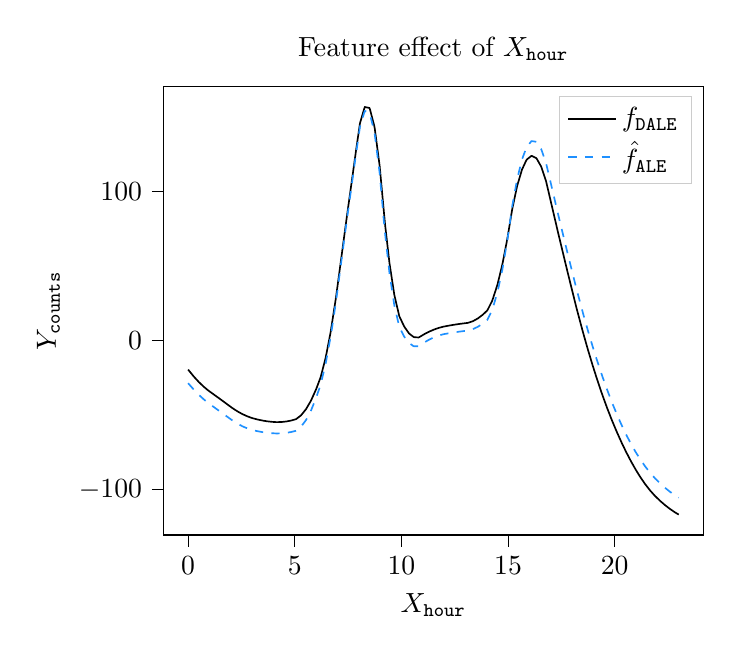
\begin{tikzpicture}

\definecolor{darkgray176}{RGB}{176,176,176}
\definecolor{dodgerblue}{RGB}{30,144,255}
\definecolor{lightgray204}{RGB}{204,204,204}

\begin{axis}[
legend cell align={left},
legend style={fill opacity=0.8, draw opacity=1, text opacity=1, draw=lightgray204},
tick align=outside,
tick pos=left,
title={Feature effect of \(\displaystyle X_{\mathtt{hour}}\)},
x grid style={darkgray176},
xlabel={\(\displaystyle X_{\mathtt{hour}}\)},
xmin=-1.15, xmax=24.15,
xtick style={color=black},
y grid style={darkgray176},
ylabel={\(\displaystyle Y_{\mathtt{counts}}\)},
ymin=-130.55351264475, ymax=170.472616656964,
ytick style={color=black}
]
\addplot [semithick, black]
table {%
0 -19.5050849914551
0.276276350021362 -24.3441772460938
0.506506443023682 -27.9236030578613
0.73673677444458 -31.0645523071289
0.943943977355957 -33.5316467285156
1.54254257678986 -39.7169952392578
2.00300312042236 -44.5988159179688
2.11811804771423 -45.7644081115723
2.32532525062561 -47.663459777832
2.55555558204651 -49.4630393981934
2.78578567504883 -50.9483070373535
2.99299287796021 -52.0300178527832
3.24624633789062 -52.9924545288086
3.47647643089294 -53.6967239379883
3.68368363380432 -54.1934471130371
3.91391396522522 -54.5767364501953
4.14414405822754 -54.7889671325684
4.37437438964844 -54.7139015197754
4.60460472106934 -54.3515357971191
4.83483505249023 -53.7018775939941
5.04204225540161 -52.8642959594727
5.06506490707397 -52.7370185852051
5.29529523849487 -50.2154121398926
5.52552556991577 -46.1370544433594
5.75575590133667 -40.5019493103027
6.00900888442993 -32.4394378662109
6.21621608734131 -24.4946517944336
6.44644641876221 -11.6443128585815
6.67667675018311 5.24092245101929
6.92992973327637 28.6440601348877
7.43643665313721 82.6207962036133
7.89689683914185 130.067947387695
8.05805778503418 145.936157226562
8.26526546478271 156.092514038086
8.28828811645508 156.789611816406
8.49549579620361 156.161087036133
8.51851844787598 155.647872924805
8.72572612762451 144.234481811523
8.74874877929688 142.510955810547
8.97897911071777 117.378860473633
9.23223209381104 78.1012954711914
9.43943977355957 52.0760345458984
9.66967010498047 30.5269412994385
9.89989948272705 16.3793964385986
10.1301298141479 9.40791988372803
10.3603601455688 4.70836496353149
10.5675678253174 2.42953133583069
10.5905904769897 2.28073143959045
10.7977981567383 2.04458355903625
10.8208208084106 2.12501859664917
11.0740737915039 4.29217100143433
11.3043041229248 5.98237943649292
11.5345344543457 7.39637041091919
11.7417421340942 8.44379425048828
11.9719715118408 9.33294486999512
12.2482481002808 10.0710592269897
12.4784784317017 10.624490737915
12.7087087631226 11.1187515258789
12.9159154891968 11.5147294998169
13.1001005172729 11.8276166915894
13.1231231689453 11.9058475494385
13.3303298950195 12.875524520874
13.3763761520386 13.199444770813
13.5835838317871 14.8272914886475
13.813814163208 17.3185062408447
14.0210208892822 20.1412181854248
14.0670671463013 21.3190975189209
14.2512512207031 26.5641231536865
14.2972974777222 28.4294090270996
14.5045042037964 37.6234588623047
14.7347345352173 51.2384872436523
14.9649648666382 68.2768707275391
15.1951951980591 88.2222595214844
15.42542552948 103.759735107422
15.6556558609009 114.889282226562
15.8628625869751 121.212203979492
15.8858861923218 121.610908508301
16.0930938720703 123.970664978027
16.1161155700684 123.936637878418
16.3233242034912 122.487854003906
16.3693695068359 121.442276000977
16.5535526275635 116.769096374512
16.6226234436035 113.865631103516
16.7837829589844 106.814399719238
16.8758754730225 101.206695556641
17.3363361358643 72.9654541015625
17.7967967987061 45.5679664611816
18.2112121582031 21.7020950317383
18.5105113983154 5.64360857009888
18.7407398223877 -5.97945785522461
18.9709701538086 -16.9456024169922
19.1781787872314 -26.2628364562988
19.4084091186523 -35.9988479614258
19.6386394500732 -45.0910110473633
19.8688697814941 -53.5393295288086
20.0990982055664 -61.3896484375
20.3293285369873 -68.7146987915039
20.5365371704102 -74.8665542602539
20.7667675018311 -81.1935348510742
20.996997833252 -86.995246887207
21.2042045593262 -91.7762222290039
21.4344348907471 -96.5489959716797
21.664665222168 -100.770584106445
21.8948955535889 -104.44100189209
22.1481475830078 -107.900184631348
22.3553562164307 -110.46851348877
22.5855846405029 -113.02222442627
22.8158149719238 -115.269233703613
23 -116.870506286621
};
\addlegendentry{$f_{\mathtt{DALE}}$}
\addplot [semithick, dodgerblue, dashed]
table {%
0 -28.6461296081543
0.299299240112305 -33.4844398498535
0.506506443023682 -36.5122833251953
0.73673677444458 -39.5242080688477
0.966966986656189 -42.1757049560547
1.74974977970123 -50.2825317382812
2.11811804771423 -54.0799827575684
2.32532525062561 -55.9247512817383
2.55555558204651 -57.6483955383301
2.78578567504883 -59.0419044494629
2.99299287796021 -60.0281982421875
3.24624633789062 -60.8593711853027
3.47647643089294 -61.46630859375
3.68368363380432 -61.8931121826172
3.91391396522522 -62.2204475402832
4.14414405822754 -62.3986968994141
4.37437438964844 -62.3219032287598
4.60460472106934 -61.990062713623
4.83483505249023 -61.4031791687012
5.04204225540161 -60.6504898071289
5.06506490707397 -60.5277214050293
5.29529523849487 -57.8714256286621
5.52552556991577 -53.4342956542969
5.75575590133667 -47.2163352966309
6.00900888442993 -38.2443809509277
6.21621608734131 -29.381742477417
6.44644641876221 -15.6827802658081
6.69969987869263 4.01029825210571
6.92992973327637 25.8215217590332
7.39039039611816 75.5200271606445
7.85085105895996 123.192329406738
8.05805778503418 143.596130371094
8.26526546478271 153.462203979492
8.28828811645508 154.119873046875
8.49549579620361 153.021850585938
8.51851844787598 152.449096679688
8.72572612762451 140.386978149414
8.74874877929688 138.58381652832
8.97897911071777 112.524017333984
9.20920944213867 75.0672760009766
9.43943977355957 45.3751182556152
9.66967010498047 23.4475517272949
9.89989948272705 9.28457546234131
10.1301298141479 2.64411807060242
10.3603601455688 -1.73881900310516
10.5675678253174 -3.74506211280823
10.5905904769897 -3.86423587799072
10.7977981567383 -3.84074091911316
10.8208208084106 -3.73213291168213
11.0740737915039 -1.27214574813843
11.3043041229248 0.624772906303406
11.5115118026733 2.059002161026
11.7417421340942 3.31951761245728
11.9719715118408 4.24510145187378
12.2482481002808 4.96000051498413
12.4784784317017 5.49322175979614
12.7087087631226 5.96644258499146
12.9159154891968 6.34280109405518
13.1001005172729 6.63770151138306
13.1231231689453 6.70726346969604
13.3303298950195 7.55532884597778
13.3763761520386 7.83442735671997
13.5835838317871 9.23264122009277
13.813814163208 11.3566951751709
14.0210208892822 13.7536668777466
14.0440444946289 14.2715625762939
14.2512512207031 20.38014793396
14.2972974777222 22.4057006835938
14.5045042037964 32.4857139587402
14.7347345352173 47.7849960327148
14.9649648666382 67.2124176025391
15.1951951980591 90.178352355957
15.42542552948 108.329772949219
15.6556558609009 121.666687011719
15.8628625869751 129.635528564453
15.9089088439941 130.593536376953
16.0930938720703 133.829193115234
16.1161155700684 133.91423034668
16.3233242034912 133.447540283203
16.3463459014893 133.071701049805
16.5535526275635 128.498184204102
16.5995998382568 126.696998596191
16.7837829589844 118.981163024902
16.8758754730225 113.421195983887
17.3363361358643 85.3754196166992
17.7967967987061 58.1768074035645
18.2112121582031 34.4831466674805
18.5335330963135 17.2674236297607
18.7407398223877 6.80826711654663
18.9709701538086 -4.24147033691406
19.2012004852295 -14.6806631088257
19.4084091186523 -23.5517692565918
19.6386394500732 -32.8170890808105
19.8688697814941 -41.4646186828613
20.0990982055664 -49.5049858093262
20.3063068389893 -56.2461433410645
20.5365371704102 -63.1648941040039
20.7667675018311 -69.4933547973633
20.9739742279053 -74.6995239257812
21.2272281646729 -80.4064331054688
21.4344348907471 -84.651123046875
21.664665222168 -88.8804550170898
21.8948955535889 -92.6121520996094
22.1481475830078 -96.1844940185547
22.3553562164307 -98.8407440185547
22.5855846405029 -101.486793518066
22.8158149719238 -103.820686340332
23 -105.487968444824
};
\addlegendentry{$\hat{f}_{\mathtt{ALE}}$}
\end{axis}

\end{tikzpicture}
}
    \resizebox{.3\columnwidth}{!}{% This file was created with tikzplotlib v0.10.1.
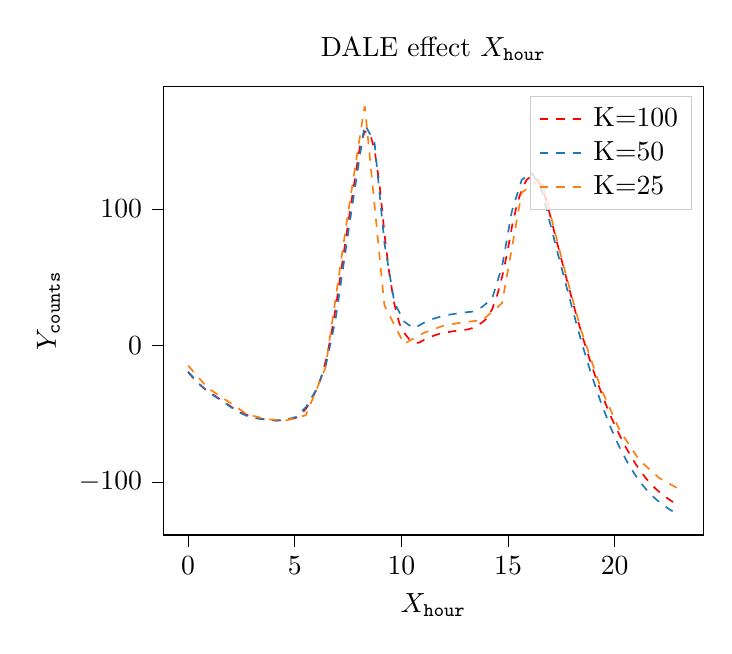
\begin{tikzpicture}

\definecolor{darkgray176}{RGB}{176,176,176}
\definecolor{darkorange25512714}{RGB}{255,127,14}
\definecolor{lightgray204}{RGB}{204,204,204}
\definecolor{steelblue31119180}{RGB}{31,119,180}

\begin{axis}[
legend cell align={left},
legend style={fill opacity=0.8, draw opacity=1, text opacity=1, draw=lightgray204},
tick align=outside,
tick pos=left,
title={DALE effect \(\displaystyle X_{\mathtt{hour}}\)},
x grid style={darkgray176},
xlabel={\(\displaystyle X_{\mathtt{hour}}\)},
xmin=-1.15, xmax=24.15,
xtick style={color=black},
y grid style={darkgray176},
ylabel={\(\displaystyle Y_{\mathtt{counts}}\)},
ymin=-138.606064986267, ymax=189.589636529361,
ytick style={color=black}
]
\addplot [semithick, red, dashed]
table {%
0 -19.5050849914551
0.276276350021362 -24.3441772460938
0.506506443023682 -27.9236030578613
0.73673677444458 -31.0645523071289
0.943943977355957 -33.5316467285156
1.54254257678986 -39.7169952392578
2.00300312042236 -44.5988159179688
2.11811804771423 -45.7644081115723
2.32532525062561 -47.663459777832
2.55555558204651 -49.4630393981934
2.78578567504883 -50.9483070373535
2.99299287796021 -52.0300178527832
3.24624633789062 -52.9924545288086
3.47647643089294 -53.6967239379883
3.68368363380432 -54.1934471130371
3.91391396522522 -54.5767364501953
4.14414405822754 -54.7889671325684
4.37437438964844 -54.7139015197754
4.60460472106934 -54.3515357971191
4.83483505249023 -53.7018775939941
5.04204225540161 -52.8642959594727
5.06506490707397 -52.7370185852051
5.29529523849487 -50.2154121398926
5.52552556991577 -46.1370544433594
5.75575590133667 -40.5019493103027
6.00900888442993 -32.4394378662109
6.21621608734131 -24.4946517944336
6.44644641876221 -11.6443128585815
6.67667675018311 5.24092245101929
6.92992973327637 28.6440601348877
7.43643665313721 82.6207962036133
7.89689683914185 130.067947387695
8.05805778503418 145.936157226562
8.26526546478271 156.092514038086
8.28828811645508 156.789611816406
8.49549579620361 156.161087036133
8.51851844787598 155.647872924805
8.72572612762451 144.234481811523
8.74874877929688 142.510955810547
8.97897911071777 117.378860473633
9.23223209381104 78.1012954711914
9.43943977355957 52.0760345458984
9.66967010498047 30.5269412994385
9.89989948272705 16.3793964385986
10.1301298141479 9.40791988372803
10.3603601455688 4.70836496353149
10.5675678253174 2.42953133583069
10.5905904769897 2.28073143959045
10.7977981567383 2.04458355903625
10.8208208084106 2.12501859664917
11.0740737915039 4.29217100143433
11.3043041229248 5.98237943649292
11.5345344543457 7.39637041091919
11.7417421340942 8.44379425048828
11.9719715118408 9.33294486999512
12.2482481002808 10.0710592269897
12.4784784317017 10.624490737915
12.7087087631226 11.1187515258789
12.9159154891968 11.5147294998169
13.1001005172729 11.8276166915894
13.1231231689453 11.9058475494385
13.3303298950195 12.875524520874
13.3763761520386 13.199444770813
13.5835838317871 14.8272914886475
13.813814163208 17.3185062408447
14.0210208892822 20.1412181854248
14.0670671463013 21.3190975189209
14.2512512207031 26.5641231536865
14.2972974777222 28.4294090270996
14.5045042037964 37.6234588623047
14.7347345352173 51.2384872436523
14.9649648666382 68.2768707275391
15.1951951980591 88.2222595214844
15.42542552948 103.759735107422
15.6556558609009 114.889282226562
15.8628625869751 121.212203979492
15.8858861923218 121.610908508301
16.0930938720703 123.970664978027
16.1161155700684 123.936637878418
16.3233242034912 122.487854003906
16.3693695068359 121.442276000977
16.5535526275635 116.769096374512
16.6226234436035 113.865631103516
16.7837829589844 106.814399719238
16.8758754730225 101.206695556641
17.3363361358643 72.9654541015625
17.7967967987061 45.5679664611816
18.2112121582031 21.7020950317383
18.5105113983154 5.64360857009888
18.7407398223877 -5.97945785522461
18.9709701538086 -16.9456024169922
19.1781787872314 -26.2628364562988
19.4084091186523 -35.9988479614258
19.6386394500732 -45.0910110473633
19.8688697814941 -53.5393295288086
20.0990982055664 -61.3896484375
20.3293285369873 -68.7146987915039
20.5365371704102 -74.8665542602539
20.7667675018311 -81.1935348510742
20.996997833252 -86.995246887207
21.2042045593262 -91.7762222290039
21.4344348907471 -96.5489959716797
21.664665222168 -100.770584106445
21.8948955535889 -104.44100189209
22.1481475830078 -107.900184631348
22.3553562164307 -110.46851348877
22.5855846405029 -113.02222442627
22.8158149719238 -115.269233703613
23 -116.870506286621
};
\addlegendentry{K=100}
\addplot [semithick, steelblue31119180, dashed]
table {%
0 -19.0568523406982
0.483483552932739 -27.5899829864502
0.943943977355957 -33.9586143493652
1.65765762329102 -41.3208885192871
2.11811804771423 -46.2027359008789
2.30230236053467 -48.1648330688477
2.76276278495789 -51.5102844238281
3.2232232093811 -53.2904281616211
3.68368363380432 -54.3948593139648
4.12112092971802 -54.8079147338867
4.14414405822754 -54.8193206787109
4.60460472106934 -54.0945930480957
5.04204225540161 -52.3263702392578
5.06506490707397 -52.1762809753418
5.52552556991577 -45.0688095092773
5.98598575592041 -32.7721710205078
6.44644641876221 -15.1332197189331
6.906907081604 18.6453113555908
7.5515513420105 87.5196990966797
8.01201248168945 134.966445922852
8.26526546478271 160.561309814453
8.28828811645508 161.809616088867
8.72572612762451 149.098709106445
8.74874877929688 147.291305541992
9.20920944213867 74.5869293212891
9.66967010498047 31.4887447357178
10.1301298141479 17.5457916259766
10.5675678253174 12.734920501709
10.5905904769897 12.6905250549316
11.0510511398315 16.6829795837402
11.5115118026733 19.7547092437744
11.9719715118408 21.9057159423828
12.4554557800293 23.2053813934326
12.8928928375244 24.1664962768555
13.3303298950195 24.9096031188965
13.3533535003662 25.0283260345459
13.7907905578613 28.3794097900391
13.8368368148804 28.9517726898193
14.2512512207031 34.5971946716309
14.2742738723755 35.4409217834473
14.7117118835449 57.6446723937988
14.757758140564 61.3840827941895
15.1721725463867 97.8089218139648
15.2182178497314 100.394157409668
15.6326322555542 120.966339111328
15.6556558609009 121.510360717773
16.0930938720703 126.492065429688
16.1161155700684 126.161819458008
16.5535526275635 115.063018798828
16.5995998382568 112.439018249512
17.2672672271729 71.3320007324219
17.7277278900146 43.8025321960449
18.1881885528564 16.976188659668
18.4644641876221 1.44218516349792
18.9019012451172 -21.0025215148926
19.362361907959 -42.0182228088379
19.8228225708008 -60.4585456848145
20.2602596282959 -75.6445541381836
20.7207202911377 -89.0095443725586
21.1811809539795 -99.7675628662109
21.6416416168213 -108.320869445801
22.1021022796631 -114.716354370117
22.5625629425049 -119.885055541992
23 -123.688079833984
};
\addlegendentry{K=50}
\addplot [semithick, darkorange25512714, dashed]
table {%
0 -14.6316518783569
0.920920848846436 -31.048433303833
1.97997999191284 -41.9419441223145
2.76276278495789 -50.2953834533691
3.68368363380432 -53.854320526123
4.58158159255981 -54.7021713256836
4.60460472106934 -54.7009506225586
5.50250244140625 -51.0714378356934
5.52552556991577 -50.791748046875
6.42342329025269 -16.8359642028809
6.44644641876221 -15.5138454437256
7.45945930480957 93.0636596679688
8.26526546478271 174.501815795898
8.28828811645508 174.671646118164
9.18618583679199 31.7446269989014
9.20920944213867 29.2628974914551
10.1071071624756 1.68466913700104
10.1301298141479 1.37699365615845
11.0510511398315 9.37294101715088
11.9719715118408 14.6067152023315
12.8928928375244 17.1037063598633
13.7907905578613 18.6290340423584
13.813814163208 18.8328590393066
14.7117118835449 31.0646076202393
14.7347345352173 32.4726219177246
15.6326322555542 111.393112182617
15.6556558609009 112.218955993652
16.5535526275635 122.44457244873
16.5765762329102 121.48802947998
17.5665664672852 60.373119354248
18.4184188842773 11.5534610748291
19.3393402099609 -30.7352237701416
20.2372379302979 -62.1434631347656
20.3753757476807 -65.432746887207
21.1581573486328 -83.8936080932617
21.2962970733643 -85.8475189208984
22.0790786743164 -96.8198623657227
22.3783779144287 -99.4268341064453
23 -104.831130981445
};
\addlegendentry{K=25}
\end{axis}

\end{tikzpicture}
}
    \resizebox{.3\columnwidth}{!}{% This file was created with tikzplotlib v0.10.1.
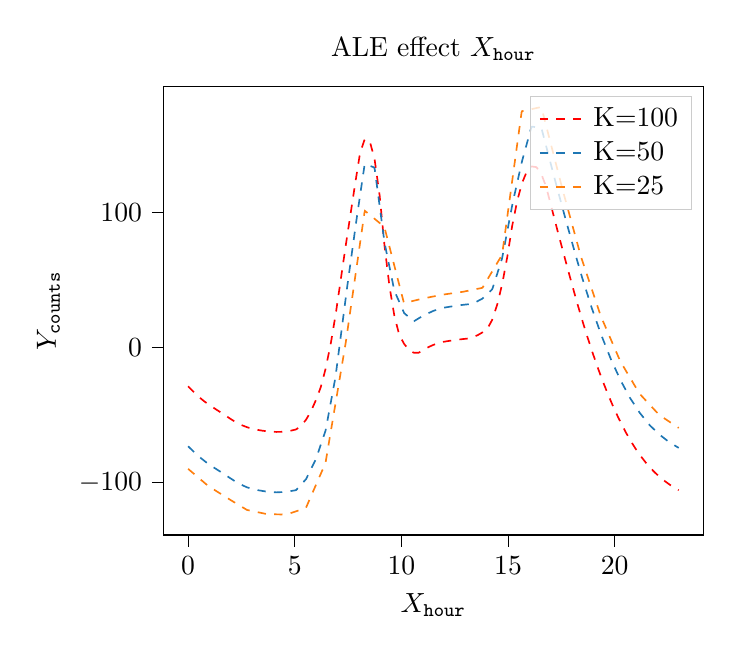
\begin{tikzpicture}

\definecolor{darkgray176}{RGB}{176,176,176}
\definecolor{darkorange25512714}{RGB}{255,127,14}
\definecolor{lightgray204}{RGB}{204,204,204}
\definecolor{steelblue31119180}{RGB}{31,119,180}

\begin{axis}[
legend cell align={left},
legend style={fill opacity=0.8, draw opacity=1, text opacity=1, draw=lightgray204},
tick align=outside,
tick pos=left,
title={ALE effect \(\displaystyle X_{\mathtt{hour}}\)},
x grid style={darkgray176},
xlabel={\(\displaystyle X_{\mathtt{hour}}\)},
xmin=-1.15, xmax=24.15,
xtick style={color=black},
y grid style={darkgray176},
ylabel={\(\displaystyle Y_{\mathtt{counts}}\)},
ymin=-138.606757724745, ymax=192.972018488682,
ytick style={color=black}
]
\addplot [semithick, red, dashed]
table {%
0 -28.6461296081543
0.299299240112305 -33.4844398498535
0.506506443023682 -36.5122833251953
0.73673677444458 -39.5242080688477
0.966966986656189 -42.1757049560547
1.74974977970123 -50.2825317382812
2.11811804771423 -54.0799827575684
2.32532525062561 -55.9247512817383
2.55555558204651 -57.6483955383301
2.78578567504883 -59.0419044494629
2.99299287796021 -60.0281982421875
3.24624633789062 -60.8593711853027
3.47647643089294 -61.46630859375
3.68368363380432 -61.8931121826172
3.91391396522522 -62.2204475402832
4.14414405822754 -62.3986968994141
4.37437438964844 -62.3219032287598
4.60460472106934 -61.990062713623
4.83483505249023 -61.4031791687012
5.04204225540161 -60.6504898071289
5.06506490707397 -60.5277214050293
5.29529523849487 -57.8714256286621
5.52552556991577 -53.4342956542969
5.75575590133667 -47.2163352966309
6.00900888442993 -38.2443809509277
6.21621608734131 -29.381742477417
6.44644641876221 -15.6827802658081
6.69969987869263 4.01029825210571
6.92992973327637 25.8215217590332
7.39039039611816 75.5200271606445
7.85085105895996 123.192329406738
8.05805778503418 143.596130371094
8.26526546478271 153.462203979492
8.28828811645508 154.119873046875
8.49549579620361 153.021850585938
8.51851844787598 152.449096679688
8.72572612762451 140.386978149414
8.74874877929688 138.58381652832
8.97897911071777 112.524017333984
9.20920944213867 75.0672760009766
9.43943977355957 45.3751182556152
9.66967010498047 23.4475517272949
9.89989948272705 9.28457546234131
10.1301298141479 2.64411807060242
10.3603601455688 -1.73881900310516
10.5675678253174 -3.74506211280823
10.5905904769897 -3.86423587799072
10.7977981567383 -3.84074091911316
10.8208208084106 -3.73213291168213
11.0740737915039 -1.27214574813843
11.3043041229248 0.624772906303406
11.5115118026733 2.059002161026
11.7417421340942 3.31951761245728
11.9719715118408 4.24510145187378
12.2482481002808 4.96000051498413
12.4784784317017 5.49322175979614
12.7087087631226 5.96644258499146
12.9159154891968 6.34280109405518
13.1001005172729 6.63770151138306
13.1231231689453 6.70726346969604
13.3303298950195 7.55532884597778
13.3763761520386 7.83442735671997
13.5835838317871 9.23264122009277
13.813814163208 11.3566951751709
14.0210208892822 13.7536668777466
14.0440444946289 14.2715625762939
14.2512512207031 20.38014793396
14.2972974777222 22.4057006835938
14.5045042037964 32.4857139587402
14.7347345352173 47.7849960327148
14.9649648666382 67.2124176025391
15.1951951980591 90.178352355957
15.42542552948 108.329772949219
15.6556558609009 121.666687011719
15.8628625869751 129.635528564453
15.9089088439941 130.593536376953
16.0930938720703 133.829193115234
16.1161155700684 133.91423034668
16.3233242034912 133.447540283203
16.3463459014893 133.071701049805
16.5535526275635 128.498184204102
16.5995998382568 126.696998596191
16.7837829589844 118.981163024902
16.8758754730225 113.421195983887
17.3363361358643 85.3754196166992
17.7967967987061 58.1768074035645
18.2112121582031 34.4831466674805
18.5335330963135 17.2674236297607
18.7407398223877 6.80826711654663
18.9709701538086 -4.24147033691406
19.2012004852295 -14.6806631088257
19.4084091186523 -23.5517692565918
19.6386394500732 -32.8170890808105
19.8688697814941 -41.4646186828613
20.0990982055664 -49.5049858093262
20.3063068389893 -56.2461433410645
20.5365371704102 -63.1648941040039
20.7667675018311 -69.4933547973633
20.9739742279053 -74.6995239257812
21.2272281646729 -80.4064331054688
21.4344348907471 -84.651123046875
21.664665222168 -88.8804550170898
21.8948955535889 -92.6121520996094
22.1481475830078 -96.1844940185547
22.3553562164307 -98.8407440185547
22.5855846405029 -101.486793518066
22.8158149719238 -103.820686340332
23 -105.487968444824
};
\addlegendentry{K=100}
\addplot [semithick, steelblue31119180, dashed]
table {%
0 -73.0295944213867
0.483483552932739 -80.3262100219727
0.943943977355957 -86.0722503662109
1.63463461399078 -93.052131652832
2.09509515762329 -97.846435546875
2.30230236053467 -100.020500183105
2.76276278495789 -103.408599853516
3.2232232093811 -105.34984588623
3.68368363380432 -106.578010559082
4.14414405822754 -107.09147644043
4.58158159255981 -106.740219116211
4.60460472106934 -106.712821960449
5.04204225540161 -105.514892578125
5.06506490707397 -105.378623962402
5.52552556991577 -97.3811645507812
5.98598575592041 -82.7204437255859
6.44644641876221 -61.2416725158691
6.906907081604 -22.0324935913086
7.45945930480957 45.1609420776367
7.89689683914185 94.8783798217773
8.26526546478271 134.32194519043
8.28828811645508 135.848922729492
8.72572612762451 133.169448852539
8.74874877929688 132.038055419922
9.20920944213867 77.4742279052734
9.66967010498047 42.0099868774414
10.1301298141479 25.4587116241455
10.5675678253174 19.581392288208
10.5905904769897 19.5158081054688
11.0510511398315 23.9011459350586
11.5115118026733 27.2109489440918
11.9719715118408 29.4452209472656
12.4554557800293 30.6770896911621
12.9159154891968 31.6511211395264
13.3303298950195 32.3632392883301
13.3533535003662 32.4914512634277
13.7907905578613 36.1472320556641
13.8368368148804 36.7766075134277
14.2512512207031 42.9912338256836
14.2742738723755 43.8286285400391
14.7117118835449 65.4701309204102
14.757758140564 69.0499725341797
15.2182178497314 107.198127746582
15.6556558609009 137.901489257812
16.0930938720703 163.001113891602
16.1161155700684 163.369003295898
16.5535526275635 162.597808837891
16.5765762329102 161.576858520508
17.2442436218262 121.308631896973
17.6816825866699 95.7949066162109
18.1421413421631 69.7332916259766
18.4644641876221 52.1377601623535
18.9249248504639 29.2084808349609
19.362361907959 9.56418228149414
19.8228225708008 -8.68426704406738
20.2832832336426 -24.4933090209961
20.7207202911377 -37.3236122131348
21.1811809539795 -48.4314765930176
21.6416416168213 -57.4496726989746
22.1021022796631 -64.4142456054688
22.5625629425049 -70.0410766601562
23 -74.1791915893555
};
\addlegendentry{K=50}
\addplot [semithick, darkorange25512714, dashed]
table {%
0 -89.7076110839844
0.943943977355957 -102.404815673828
1.97997999191284 -112.664199829102
2.76276278495789 -120.120399475098
3.68368363380432 -123.145240783691
4.58158159255981 -123.534996032715
4.60460472106934 -123.51879119873
5.50250244140625 -118.79963684082
5.52552556991577 -118.507827758789
6.42342329025269 -86.0327835083008
6.44644641876221 -84.83203125
7.39039039611816 3.69972920417786
8.26526546478271 99.6076049804688
8.28828811645508 101.115272521973
9.18618583679199 89.4567947387695
9.20920944213867 88.7125854492188
10.1071071624756 33.6399116516113
10.1301298141479 32.8881683349609
11.0510511398315 36.4285697937012
11.9719715118408 39.2134017944336
12.8928928375244 41.2662658691406
13.7907905578613 44.1628112792969
13.813814163208 44.5594520568848
14.7117118835449 68.4099655151367
14.7347345352173 70.3300552368164
15.6326322555542 173.919738769531
15.6556558609009 174.823348999023
16.5535526275635 177.900253295898
16.5765762329102 176.900024414062
17.5665664672852 116.187698364258
18.4184188842773 67.2121658325195
19.3393402099609 23.6039810180664
20.2602596282959 -10.096302986145
21.1581573486328 -34.0074882507324
21.3193187713623 -36.7692565917969
22.0790786743164 -49.7056350708008
22.3783779144287 -52.8796615600586
23 -59.459545135498
};
\addlegendentry{K=25}
\end{axis}

\end{tikzpicture}
}
    \caption{Feature effect plots on \(X_{\texttt{hour}}\): (Left)
      DALE vs ALE for \(K=200\). (Center) DALE plots for
      \(K = \{25, 50, 100\}\). (Right) ALE plots for
      \(K = \{25, 50, 100\}\)}
  \label{fig:bike-sharing-feature-3}
\end{figure}


\begin{table}
  \caption{Evaluation of DALE and ALE approximation when lowering the
    number of bins \(K\). The ground-truth effect has been computed
    for \(K=200\).}
  \label{tab:bike-sharing-accuracy}
  \centering
  \begin{tabular}{c|c|c|c|c|c}
    \multicolumn{6}{c}{Accuracy on Bike-Sharing Dataset - Feature \(X_{\mathtt{hour}}\)} \\
    \hline \hline
    & & \multicolumn{4}{|c}{Number of bins} \\
    \hline
    & & 100 & 50 & 25 & 15 \\
    \hline
    \hline
    \multirow{2}{*}{\(\mathtt{NMSE}\)} & \(\dale\) & \textbf{0.007} & \textbf{0.01} & \textbf{0.03} & \textbf{0.09} \\
    & \(\alep\) & 0.04 & 0.43 & 0.79 & 0.83 \\
    \hline
  \end{tabular}
\end{table}
